\documentclass[a4paper,zihao=-4,linespread=1]{ctexart}

%\setmainfont{Times New Roman}
%\setCJKmainfont{SimSun}  % 设置正文字体为宋体% SimSun 是宋体的字体名称

\usepackage{listings}%列代码使用

\usepackage{graphicx}  % 引入图形包,用于插入图片
\newcommand{\fig}[3]%快速插入图的命令
{
    \begin{figure}[htp]
        \centering
        \caption{#1}
        \includegraphics[width=#2\textwidth]{#3}
    \end{figure}
}
\newcommand{\figu}[2]%快速插入图的命令
{
    \begin{figure}[htp]
        \centering
        \includegraphics[width=#1\textwidth]{#2}
    \end{figure}
}
\newcommand{\bold}[1]{\textbf{#1}}%加粗命令


\usepackage{geometry}  % 引入页面布局包,用于调整页面尺寸
\geometry{a4paper, scale=0.8}  % 设置页面尺寸和边距

%\usepackage{mathptmx}  % 使用 Times 字体的数学版本


\usepackage[]{indentfirst}          % 强制段首缩进
\usepackage[]{bm}               %用于生成数学环境中的粗体符号。
\usepackage{amsmath}          %提供了丰富的数学功能和环境,用于改善数学公式的排版和书写。
\allowdisplaybreaks[1]          %它接受一个可选参数,取值范围为 0 到 4,参数值越大,公式换行的灵活性越高。

\usepackage{natbib}  % 使用 natbib 包来处理引用
\setcitestyle{numbers,square}
% 改变引用字体
\renewcommand{\bibfont}{\zihao{-4}\songti}

\usepackage[dvipsnames]{xcolor} %用到的彩色
\usepackage{tcolorbox}      %彩色盒子
\tcbuselibrary{breakable}  % 支持分页
\tcbuselibrary{skins}      % 支持更多样式
\newtcolorbox[]{py}[1][]{colback=SeaGreen!10!CornflowerBlue!10,colframe=RoyalPurple!55!Aquamarine!100!,breakable, enhanced jigsaw}

\newtcolorbox[]{code}[2][]{title=\textbf{#2},colback=SeaGreen!10!CornflowerBlue!10,colframe=RoyalPurple!55!Aquamarine!100!,breakable, enhanced jigsaw}

\definecolor{safecolor}{rgb}{0.2, 0.4, 0.8}
\newtcolorbox[]{define}[2][]
{enhanced,
left=22pt,right=22pt,
fonttitle=\bfseries\large,
coltitle=white,%%%文字色
colbacktitle=blue!50!black,%%%背景色
attach boxed title to top left={},%%%微調整
boxed title style={skin=enhancedfirst jigsaw,arc=1mm,bottom=0mm,boxrule=0mm},%装飾
boxrule=0.5pt,
colback=safecolor!5!,%%%本文背景色
colframe=safecolor,%%%本文枠色
sharp corners=northwest,%%%左上角調整 
drop fuzzy shadow,
breakable,
title=\vspace{3mm}#2,
arc=1mm,%弧
#1}

\usepackage{titlesec}

\usepackage{hyperref}  % 可选,用于生成超链接

%\usepackage[braket, qm]{qcircuit}%量子线路包1 
%\def\ingate{\vbox to 3.5em{\hbox to 4em{\tiny$x$\hss $x$}\vss
%  \hbox to 4em{\Large\hss$U_f$\hss}\vss
%  \hbox to 4em{\medmuskip1mu\tiny$y$\hss $y\oplus f(x)$}\vskip-2pt}}

\usepackage{tikz}
\usetikzlibrary{quantikz2}%量子线路包2

\usepackage{enumitem}%列表环境
% 定义新的列表环境
\newlist{paralist}{itemize}{1}
\setlist[paralist]{label=$\bullet$, leftmargin=38pt, itemindent=0pt, labelindent=0pt}
\begin{document}

\begin{titlepage}
    \centering  % 使封面内容居中
    \vspace*{5cm}  % 在页面顶部添加一些垂直空间

    \textbf{\LARGE 量子算法与量子计算的原理、实现与展望}  % 封面标题,使用大号加粗字体

    \vspace{1cm}  % 添加一些垂直空间
    \large 量子科技导论结课论文  % 副标题
    
    \vspace{8cm}  % 添加垂直空间

    \large lhn % 作者名字

    \vspace{0.5cm}  % 添加垂直空间
    \large \today  % 日期
    \vfill   % 填充剩余空间,使内容在页面上分布更均匀
    
\includegraphics[width=0.4\textwidth]{figures/lzu2020.png}  % 插入图片,调整图片宽度


\end{titlepage}

\thispagestyle{empty}  % 去掉前言部分的页码
\setcounter{page}{0}
\section*{摘要}
本文系统研究了量子计算的基本原理、实现方法及量子算法的编程实现。

首先,论文从量子计算基础原理出发,介绍了量子计算的核心概念,包括量子位的特性、量子门的分类与作用以及量子线路、量子算法的概念。

接着,论文探讨了量子计算的物理实现方式,通过阅读相关综述,分析了离子阱量子计算和超导量子计算的原理、优势及面临的挑战。

最后,在量子算法部分,论文详细介绍了Deutsch-Jozsa算法和Grover搜索算法的理论基础,并利
用Qiskit框架在经典计算机上进行了模拟实现,验证了算法的正确性和有效性。

在附录部分,论文总结了Qiskit框架的搭建及使用方法,并对量子编程语言和量子云平台进行了概述。

\bold{关键词:量子计算、量子算法、量子计算的物理实现、Qiskit}
\thispagestyle{empty}
\setcounter{page}{0}
\thispagestyle{empty}
\setcounter{page}{0}

\tableofcontents  % 生成目录
\setcounter{page}{0}
\section{引言}
\subsection{选题背景}
随着量子力学理论的不断发展和计算科学的深入探索,量子计算作为一种新兴的计算范式,逐渐成为学术界和工业界的热点研究领域。量子计算利用量子比特(qubit)的叠加和纠缠特性,能够在某些特定问题上实现指数级的加速,展现出超越传统经典计算的强大潜力。例如,Shor算法能够在多项式时间内分解大整数,对现代密码学构成潜在威胁;而Grover搜索算法则为无序数据库搜索问题提供了平方加速的解决方案。这些突破性进展不仅推动了理论物理学的发展,也为计算机科学、信息科学、化学和材料科学等领域带来了新的机遇和挑战。

\subsection{结构安排}
文章的结构安排如下:

\begin{itemize}
    \item \textbf{第1章:引言} \\
    本章介绍了量子计算的研究背景、意义以及本文的研究目标和结构安排。
    
    \item \textbf{第2章:量子位、量子门、量子线路} \\
    本章详细介绍了量子计算的基础概念,包括量子位的特性、量子门的分类与作用以及量子线路的设计原理。通过数学描述和物理实现的结合,为后续章节奠定理论基础。
    
    \item \textbf{第3章:量子计算物理实现} \\
    本章探讨了量子计算的物理实现方法,总结了离子阱量子计算和超导量子计算的原理、优势及面临的挑战。
    
    \item \textbf{第4章:量子算法及编码实现} \\
    本章详细介绍了Deutsch-Jozsa算法和Grover搜索算法的理论基础,并利用Qiskit框架在经典计算机上进行了模拟实现。通过编程实践,验证了这些量子算法的正确性和有效性,同时展示了量子编程的基本方法和流程。
    
    \item \textbf{第5章:总结} \\
    本章对全文进行了总结,回顾了量子计算的基本原理和实现方法,并展望了量子计算未来的发展方向。同时,本文还强调了量子编程语言和量子云平台在量子计算研究和应用中的重要作用。
\end{itemize}
\subsection{研究意义}
本文旨在系统总结量子计算的基本原理、实现方法以及量子算法的编程实现。通过深入探讨量子计算的核心概念,如量子位的特性、量子门的作用以及量子线路的设计,本文为读者提供了一个详实的量子计算入门框架。同时,本文还分析了量子计算的物理实现方式,包括离子阱量子计算和超导量子计算的原理、优势及面临的挑战。最后,本文通过Qiskit框架在经典计算机上对Deutsch-Jozsa算法和Grover搜索算法进行了模拟实现,验证了这些量子算法的正确性和有效性。这些研究不仅有助于加深对量子计算的理解,也为量子编程和量子算法的实际应用提供了实践指导。

通过本文的研究,读者可以了解量子计算的基本原理、物理实现以及量子算法的编程实践,为进一步探索量子计算的前沿领域提供理论支持和实践指导。
\thispagestyle{empty}
\setcounter{page}{0}
\section{量子位、量子门、量子线路}
\subsection{量子位}
比特是所有计算的基础。无论是录制数字视频、制作 3D 模型动画还是使用计算器应用程序,从操作系统到软件的所有数据均由二进制代码构建,二进制代码是比特的集合。计算机字节由八个比特组成,这是使用二进制表达一个文本字符所需的最少比特数。任意\textbf{两级系统},如果系统的状态只能是两个状态之一(例如,上或下,左或右,打开或关闭),均可用于表示一个比特。

在传统或经典计算中,可以将单个比特视为一段二进制信息,表示为 0 或 1。现代计算机里比特通常由电压或电流脉冲(或触发器电路的状态)表示。当这些系统中没有电流流动时,可将电路视为关闭,此状态表示为 0。当有电流流动时,可将电路视为开启,此状态表示为 1。

与经典位不同,量子位编码在量子态上,由于态的叠加性,除了0或1之外,它还可能处于0与1的叠加态。

\begin{define}{量子位(Quantum bit)}
在量子信息理论中,量子位(Qubit)是量子信息的基本单位,类似于经典计算中的比特(Bit)。然而,量子位与经典比特有着本质的不同。经典比特只有两种状态:0 和 1,而量子位可以同时处于 0 和 1 的叠加态。量子位是一个量子系统,其中布尔状态 0 和 1 由一对归一化且相互正交的量子基态表示。

 数学上,量子位的状态可以表示为:
     \[
     |\psi\rangle = \alpha |0\rangle + \beta |1\rangle
     \]
其中,\(\alpha\) 和 \(\beta\) 是复数,满足归一化条件:
     \[
     |\alpha|^2 + |\beta|^2 = 1
     \]
\(\alpha\) 和 \(\beta\) 分别表示量子位处于状态 \(|0\rangle\) 和 \(|1\rangle\) 的概率幅。
\end{define}
量子位可以由任何具有量子现象的粒子、亚粒子或准粒子实现。例如,超导量子位、离子阱量子位、拓扑量子位和光量子位等。这些物理系统可以实现量子位的初始化、操作和测量。

量子位可以处于任意的叠加态,这使得量子计算能够进行并行计算。例如,一个量子位可以处于:
     \[
     |\psi\rangle = \alpha|0\rangle + \beta |1\rangle
     \]
测量量子位时,其状态会坍缩为 0 或 1,概率分别为 \(|\alpha|^2\) 和 \(|\beta|^2\)。

 多个量子位可以形成量子纠缠态,这种状态下,量子位之间的状态不再是独立的,而是相互关联的。例如,两个量子位可以形成Bell态:
     \[
     |\Phi^+\rangle = \frac{1}{\sqrt{2}} (|00\rangle + |11\rangle)
     \]
在这种纠缠态下,测量其中一个量子位的状态会立即确定另一个量子位的状态,无论它们相距多远。

量子位的状态可以几何地表示为Bloch球上的一个点。Bloch球是一个单位球,其表面的点对应于量子位的所有可能状态。量子位的状态可以表示为:
     \[
     |\psi\rangle = \cos\left(\frac{\theta}{2}\right) |0\rangle + e^{i\phi} \sin\left(\frac{\theta}{2}\right) |1\rangle
     \]
其中,\(\theta\) 和 \(\phi\) 分别是极角和方位角。

量子位是量子计算的基本信息单元,具有量子叠加和量子纠缠的特性。通过数学表示,量子位的状态可以用二维复数向量描述,满足归一化条件。量子位的物理实现方式多样,包括超导量子位、离子阱量子位、拓扑量子位和光量子位等。量子位的测量是一个随机过程,测量结果会使其状态坍缩到 0 或 1。这些特性使得量子位在量子计算中具有巨大的潜力和应用价值。

\subsection{量子门}
量子门(Quantum Gate)是量子计算中的基本操作单元,通过幺正矩阵表示的线性变换改变量子位的状态。量子门是可逆的,可以组合成复杂的量子线路,实现量子算法。常见的量子门包括Hadamard门、Pauli-X门、Pauli-Y门、Pauli-Z门和CNOT门等。这些量子门在量子计算中具有重要的作用,是实现量子算法的基础。
\begin{define}{量子门(Quantum Gate)}
     量子门是量子计算中的基本操作单元,类似于经典计算中的逻辑门。量子门通过对量子位进行线性变换来改变其状态。量子门是可逆的,这意味着每个量子门都有一个逆门。

     量子门可以用一个幺正矩阵(Unitary Matrix)表示。对于一个作用在单个量子位上的量子门,其矩阵表示为一个 2x2 的幺正矩阵 \(U\),满足 \(U^\dagger U = I\),其中 \(U^\dagger\) 是 \(U\) 的共轭转置,\(I\) 是单位矩阵。矩阵的幺正性满足变换后态保持归一化。
\end{define}

\subsubsection{一位门}
\begin{figure}[htbp]
     \centering
     \caption{一位量子门}
     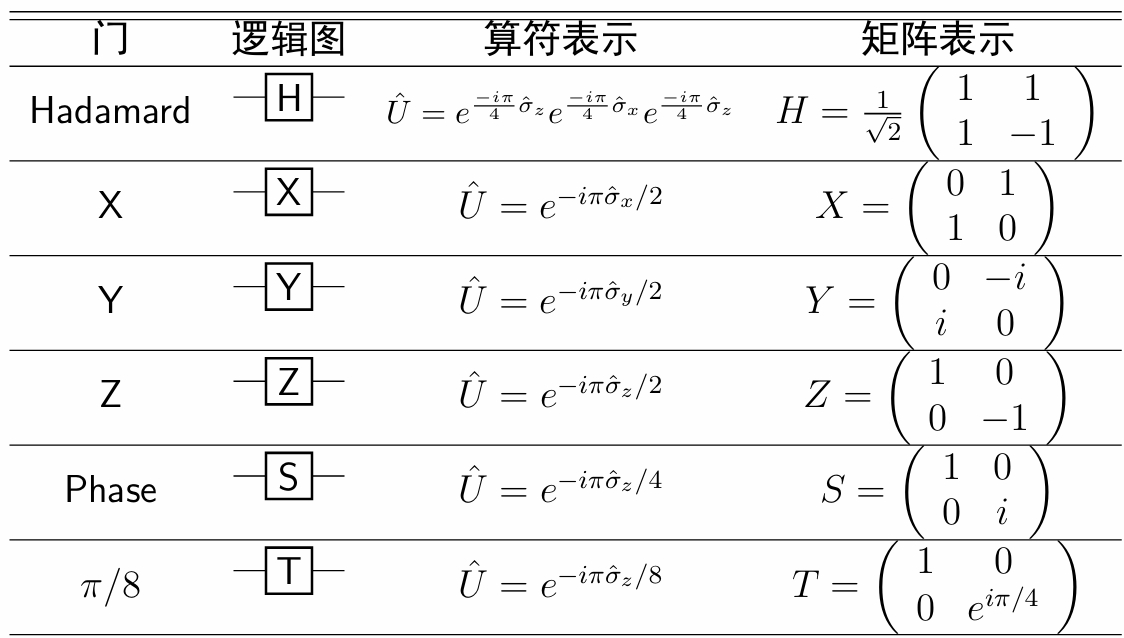
\includegraphics[width=0.8\textwidth]{figures/onedoor.png}
\end{figure}
\textbf{1. Hadamard门(H门)}

\begin{center}
     \begin{quantikz}
          \qw & \gate{H} & \qw \\
     \end{quantikz}
\end{center}


矩阵表示:
     \[
     H = \frac{1}{\sqrt{2}} \begin{pmatrix} 1 & 1 \\ 1 & -1 \end{pmatrix}
     \]

Hadamard门简称H门。H门作用在单量子比特上,将基态\(|0\rangle\)变成\((|0\rangle+|1\rangle)/\sqrt{2}\),将\(|1\rangle\)变成\((|0\rangle-|1\rangle)/\sqrt{2}\),即
     \[
     H|0\rangle = \frac{1}{\sqrt{2}} (|0\rangle + |1\rangle)
     \]
     \[
     H|1\rangle = \frac{1}{\sqrt{2}} (|0\rangle - |1\rangle)
     \]

H门通常用作以下用途:
1. 基变换
2. 将多个量子比特的初态制备为等权叠加态\( H^{\otimes n} \) 作用在零态 \( |0\rangle^{\otimes n} \) 上能够产生等权叠加态\( \frac{1}{\sqrt{2^n}} \sum_{x \in \{0,1\}^n} |x\rangle \)即从零态得到 \( 2^n \) 个态的叠加态。


\textbf{2. Pauli-X门(X门)}

\begin{center}
     \begin{quantikz}
          \qw & \gate{X} & \qw \\
     \end{quantikz}
\end{center}



矩阵表示:
     \[
     X = \begin{pmatrix} 0 & 1 \\ 1 & 0 \end{pmatrix}
     \]

 类似于经典计算中的NOT门,将 \(|0\rangle\) 变为 \(|1\rangle\),将 \(|1\rangle\) 变为 \(|0\rangle\)。
     \[
     X|0\rangle = |1\rangle
     \]
     \[
     X|1\rangle = |0\rangle
     \]

\textbf{3. Pauli-Y门(Y门)}

\begin{center}
     \begin{quantikz}
          \qw & \gate{Y} & \qw \\
     \end{quantikz}
\end{center}


矩阵表示:
     \[
     Y = \begin{pmatrix} 0 & -i \\ i & 0 \end{pmatrix}
     \]
     
类似于X门,但带有相位变化。
     \[
     Y|0\rangle = i|1\rangle
     \]
     \[
     Y|1\rangle = -i|0\rangle
     \]

\textbf{4. Pauli-Z门(Z门)}

\begin{center}
     \begin{quantikz}
          \qw & \gate{Z} & \qw \\
     \end{quantikz}
\end{center}


矩阵表示:
     \[
     Z = \begin{pmatrix} 1 & 0 \\ 0 & -1 \end{pmatrix}
     \]

对量子位的相位进行变化,但不改变其概率幅。
     \[
     Z|0\rangle = |0\rangle
     \]
     \[
     Z|1\rangle = -|1\rangle
     \]

\textbf{5. Phase门(S门)}

\begin{center}
     \begin{quantikz}
          \qw & \gate{S} & \qw \\
     \end{quantikz}
\end{center}


矩阵表示:
     \[
     S = \begin{bmatrix} 1 & 0 \\ 0 & i \end{bmatrix} = \begin{bmatrix} 1 & 0 \\ 0 & e^{i(\pi/2)} \end{bmatrix}
     \]

S门相当于绕布洛赫球z轴逆时针旋转 \(\pi/2\) 角度。布洛赫球上任一量子态 \(|\psi\rangle = \cos\frac{\theta}{2}|0\rangle + e^{i\varphi}\sin\frac{\theta}{2}|1\rangle\),其中 \(e^{i\varphi}\) 是相对相位,\(\varphi\) 是相位角。S门作用后,相位角由 \(\varphi\) 变为 \(\varphi + \pi/2\)。

对于任意量子态\(|\psi\rangle = \alpha|0\rangle + \beta|1\rangle\),S门作用后得到的新的量子态为
     \[
     S|\psi\rangle = \begin{bmatrix} 1 & 0 \\ 0 & i \end{bmatrix} \begin{bmatrix} \alpha \\ \beta \end{bmatrix} = \alpha|0\rangle + i\beta|1\rangle
     \]

\textbf{6. \(\pi/8\)门(T门)}

\begin{center}
     \begin{quantikz}
          \qw & \gate{T} & \qw \\
     \end{quantikz}
\end{center}


矩阵表示:
     \[
     T = \begin{bmatrix} 1 & 0 \\ 0 & e^{i(\pi/4)} \end{bmatrix} 
     \]

 T门相当于绕布洛赫球z轴逆时针旋转 \(\pi/4\) 角度,有时也称之为 \(\pi/8\) 门。
     \[ 
     T = \begin{bmatrix} 1 & 0 \\ 0 & e^{i(\pi/4)} \end{bmatrix} = e^{i(\pi/8)} \begin{bmatrix} e^{-i(\pi/8)} & 0 \\ 0 & e^{i(\pi/8)} \end{bmatrix} 
     \]

上式方括号外的 \(e^{i(\pi/8)}\) 对T门作用后的结果观测不起作用。将T门作用两次等于作用一次S门,即 \(S = TT\)。

 T门作用在任意量子态 \(|\psi\rangle = \alpha|0\rangle + \beta|1\rangle\) 上,得到的新的量子态为
     \[ 
     T|\psi\rangle = \begin{bmatrix} 1 & 0 \\ 0 & e^{i(\pi/4)} \end{bmatrix} \begin{bmatrix} \alpha \\ \beta \end{bmatrix} = \begin{bmatrix} \alpha \\ e^{i(\pi/4)}\beta \end{bmatrix} = \alpha|0\rangle + e^{i(\pi/4)}\beta|1\rangle 
     \] 

\subsubsection{多位门}

\textbf{1. 受控非门(CNOT门)}
\begin{center}
     \begin{quantikz}
          \qw & \ctrl{1} & \qw \\
          \qw & \targ{} & \qw
      \end{quantikz}
\end{center}
受控非门又称CX门或CNOT门,为双量子比特门,其中一个输入为控制量子比特,另一个输入为目标量子比特。当控制量子比特为 \(|1\rangle\) 时,目标量子比特执行X门操作,否则保持不变。

矩阵表示(高位为控制量子比特):
     \[
     \text{CNOT} = \begin{pmatrix} 1 & 0 & 0 & 0 \\ 0 & 1 & 0 & 0 \\ 0 & 0 & 0 & 1 \\ 0 & 0 & 1 & 0 \end{pmatrix}
     \]

作用效果:
     \[
     \text{CNOT}(|00\rangle) = |00\rangle
     \]
     \[
     \text{CNOT}(|01\rangle) = |01\rangle
     \]
     \[
     \text{CNOT}(|10\rangle) = |11\rangle
     \]
     \[
     \text{CNOT}(|11\rangle) = |10\rangle
     \]

\textbf{2. 互换门(SWAP门)}
\begin{center}
     \begin{quantikz}
         \qw & \swap{1} & \qw \\
         \qw & \targX{} & \qw
     \end{quantikz}    
 \end{center}

矩阵表示:
\[
\text{SWAP} = \begin{bmatrix}
1 & 0 & 0 & 0 \\
0 & 0 & 1 & 0 \\
0 & 1 & 0 & 0 \\
0 & 0 & 0 & 1
\end{bmatrix}
\]

对于任意两个量子比特的组合状态,如\(|00\rangle\)、\(|01\rangle\)、\(|10\rangle\)和\(|11\rangle\),SWAP门将分别使它们变为\(|00\rangle\)、\(|10\rangle\)、\(|01\rangle\)和\(|11\rangle\)。SWAP门会交换量子态\(|01\rangle\)和\(|10\rangle\)的状态,而量子态\(|00\rangle\)和\(|11\rangle\)保持不变。

\textbf{3.控制控制非门(Toffoli门)}

\begin{center}
     \begin{quantikz}
      \qw   & \ctrl{1} & \qw \\
      \qw   & \ctrl{1} & \qw \\
      \qw   & \targ{}    & \qw \\
     \end{quantikz}    
 \end{center}

Toffoli门,也称为控制控制非门(Controlled-Controlled-NOT,简称CCNOT),是一种三比特量子门。这种门有两个控制位和一个目标位。当两个控制位都为1时,Toffoli门会对目标位执行NOT操作,即翻转目标位的量子态;如果任一控制位为0,则目标位保持不变。Toffoli门的矩阵表示为一个8×8的矩阵,作用于三比特量子态。

当 \(|q_2 q_1 q_0\rangle\) 中的 \(q_0\) 和 \(q_1\) 为控制量子比特,\(q_2\) 为目标量子比特时,其矩阵表示为:
\[ \text{CCX}_{q_0, q_1, q_2} = I \otimes I \otimes |0\rangle\langle 0| + \text{CX}_{q_1, q_2} \otimes |1\rangle\langle 1| \]

\[ = \begin{bmatrix} 1 & 0 & 0 & 0 & 0 & 0 & 0 & 0 \\ 0 & 1 & 0 & 0 & 0 & 0 & 0 & 0 \\ 0 & 0 & 1 & 0 & 0 & 0 & 0 & 0 \\ 0 & 0 & 0 & 0 & 0 & 0 & 0 & 1 \\ 0 & 0 & 0 & 0 & 1 & 0 & 0 & 0 \\ 0 & 0 & 0 & 0 & 0 & 1 & 0 & 0 \\ 0 & 0 & 0 & 0 & 0 & 0 & 1 & 0 \\ 0 & 0 & 0 & 1 & 0 & 0 & 0 & 0 \end{bmatrix} \]

\subsection{量子线路}
量子线路是实现量子算法的基础。量子线路通过一系列量子门来操作量子位,这些量子位是量子计算的基本单元,可以处于叠加态和纠缠态。
\begin{define}{量子线路(Quantum Circuit)}
     量子线路(Quantum Circuit),也称为量子电路或量子门电路,是量子计算中用于描述量子算法的一种图形化表示方法。它类似于经典计算中的逻辑电路,但专门用于处理量子信息。
\end{define}
量子线路的一个例子:
\begin{center}
     \begin{quantikz}
          \lstick{$\ket{0}$} && \ctrl{1} & \targ{} & \swap{1} & \ctrl[vertical
          wire=c]{2} &&\\
          \lstick{$\ket{0}$} && \control{} & \ctrl[open]{-1} & \targX{} && \gate{X} &\\
          \lstick{$\ket{0}$} &&&& \gate{U} & \meter{} \wire[u][1]{c}
     \end{quantikz}  
\end{center}

\subsection{量子算法}
量子算法是利用量子计算原理进行的计算方法,它能够在特定问题上比经典算法更高效地解决复杂计算任务。与传统计算机使用的经典比特不同,量子比特可以同时处于多种状态,利用叠加和纠缠现象,使得量子计算机能够在进行大规模计算时展现出超越经典计算机的潜力。具体来说,许多需要指数级时间才能解决的问题,在量子算法的帮助下,可以在多项式时间内完成。例如,Shor算法能够有效地分解大整数,从而在加密领域带来革命性的影响。
\begin{define}{量子算法}
    量子算法是运行在量子计算机上的算法,利用量子的特性,如态叠加、量子纠缠等,来解决特定问题。与经典算法相比,量子算法在某些情况下能够显著提高计算速度和效率,解决一些经典计算机难以解决的问题。
\end{define}




\section{量子计算物理实现}
\subsection{离子阱量子计算}
离子阱量子计算是一种利用囚禁离子作为量子比特(qubit)进行量子信息处理的技术。它是量子计算领域中最具前景的方法之一,具有高保真度、长相干时间和精确控制等优势。
\subsubsection{量子位的物理实现}
在基于离子阱的量子计算中,存在两种不同类型的量子位实现方式:(1.)基态量子位,其中信息被编码在基态的两个超精细或塞曼子能级中,以及(2.)光学量子位,其中信息被编码在基态和光学可及的亚稳态激发态中。这两种类型的量子位需要不同的实验技术,特别是基态量子位通过双光子拉曼跃迁或直接微波激发来操纵。相比之下,对光学量子位的操作是通过激光器提供的共振光场来执行的。测量寄存器中量子位的状态通常通过电子搁置方法进行,对两种类型的量子位都使用辅助的短寿命状态。

为了实现量子算法,量子位必须在明确定义的状态下初始化。对于原子,通常可以通过光学泵(optical pumping)方便地实现这一点。光学泵的基本原理是将原子驱动到驱动不再作用的状态。通常使用圆偏振光将原子泵到极端的塞曼能级之一。目标状态在不到1微秒内被占据的概率大于0.99。初始化保真度通常受到驱动激光沿量子比特优选轴的偏振质量的限制。

在量子算法结束时,量子寄存器需要被测量。通过仅与量子比特的一个能级耦合的辐射可以实现这一点。

\subsubsection{量子门的物理实现}
所有量子算法都可以分解为一系列单量子比特操作加上一个特定的双量子比特操作,例如条件相位门、受控非门或 SWAP 门。

\bold{1.单量子门}

单量子门作用于量子比特上对应于态矢在布洛赫球进行的旋转。
通过两个量子比特能级之间的拉比翻转实现单量子比特操作。数学上,可以利用旋转 $R^C(\theta, \varphi)$ 作用于状态向量 $\alpha |0\rangle + \beta |1\rangle$来描述共振辐射诱导的耦合效应。

\[
R^C(\theta, \varphi) = \exp \left( i \frac{\theta}{2} \left( e^{i \varphi} \sigma_+ + e^{-i \varphi} \sigma_- \right) \right) = I \cos \frac{\theta}{2} + i (\sigma_x \cos \varphi - \sigma_y \sin \varphi) \sin \frac{\theta}{2}
\]
\[
= \begin{pmatrix} \cos \frac{\theta}{2} & i e^{i \varphi} \sin \frac{\theta}{2} \\ i e^{-i \varphi} \sin \frac{\theta}{2} & \cos \frac{\theta}{2} \end{pmatrix},
\]

其中 $\sigma_+ = \begin{pmatrix} 0 & 0 \\ 0 & 0 \end{pmatrix}$ 和 $\sigma_- = \begin{pmatrix} 0 & 0 \\ 0 & 0 \end{pmatrix}$ 是相应的原子激发和湮灭算符。$\sigma_x = \begin{pmatrix} 0 & 0 \\ 0 & 0 \end{pmatrix}$ 和 $\sigma_y = \begin{pmatrix} 0 & -i \\ i & 0 \end{pmatrix}$ 是泡利自旋矩阵。角度 $\theta$ 和 $\varphi$ 指定旋转。
任何 $\sigma_x$ 和 $\sigma_y$ 操作的线性组合都可以通过激光脉冲实现。绕 z 轴的旋转可以分解为绕 x 轴和 y 轴的旋转。
通过调整激光脉冲,可以在布洛赫球上实现任意旋转,从而操控量子态实现任意的单量子门。

\bold{2.双量子门}

Cirqac-Zoller门:

Cirqac 和 Zoller 提出了在离子串中两个离子之间执行双量子比特门的以下过程:首先,第一个量子比特的量子信息被转移到离子晶体的模式(the bus mode)的运动自由度中。由此产生的运动状态不仅影响被寻址的离子本身,还影响整个离子串。因此,在第二个离子上,可以执行以离子串的运动状态为条件的操作。最后,量子信息被映射回第一个离子的量子比特上。利用Cirqac-Zoller门可以得到普通的受控非门或零受控非操作。


M\o{}lmer-S\o{rensen} 门:

利用双色激光场,通过调整激光频率接近集体模式的红边带和蓝边带,实现量子比特之间的纠缠。

基本原理如下:两个离子都受到双色激光场的照射,频率为 $\omega_0 \pm (\omega_{\text{qubit}} + \delta)$,分别调谐接近集体模式的红边带和蓝边带。这两个频率的总和是量子比特频率 $\omega_{\text{qubit}}$ 的两倍,然而,每个激光场本身并不谐振于任何能级。因此,两个离子只能集体改变它们的状态,并适当选择相互作用时间,实现动力学

\[
\begin{array}{l}
|ee\rangle \rightarrow (|ee\rangle + i|gg\rangle)/\sqrt{2} \\
|eg\rangle \rightarrow (|eg\rangle + i|ge\rangle)/\sqrt{2} \\
|ge\rangle \rightarrow (|ge\rangle + i|eg\rangle)/\sqrt{2} \\
|gg\rangle \rightarrow (|gg\rangle + i|ee\rangle)/\sqrt{2}
\end{array}
\] 

通过引入新基 $\ket{\pm}_i = (\ket{e}_i \pm \ket{g}_i)/\sqrt{2}$,$\ket{\pm}$ 是方程 (15) 描述的酉操作的本征态,并通过门的作用转换为 $\ket{++} \rightarrow \ket{++}, \ket{+-} \rightarrow i\ket{+-}, \ket{-+} \rightarrow i\ket{-+}, \ket{--} \rightarrow \ket{--}$,省略了相位因子 $e^{-i\pi/4}$。


Geometric phase门:

通过激光场对离子施加依赖于电子态的力,使得不同电子态获得不同的相位,从而实现量子门操作。

Geometric phase门也使用两个激光场同时照射多个离子。施加一个依赖于电子态的力,使得对于不同的电子态获得不同的相位。两个激光频率的差异调谐接近于轴频率之一,形成驻波。选择离子之间的距离,使得每个离子在给定时间内经历驻波的相同相位,如果它们具有相同的电子态,则离子被推在同一方向上。如果离子处于不同的电子态,则作用于离子上的力不同,可以激发呼吸模式(breathing mode)。从运动模式的驱动失谐选择使得运动和驱动之间的相位在门时间的一半后改变符号。通过这种方式,离子串在完整的门时间后被驱动回到原始运动状态。这确保在门操作后运动与电子态解耦合。与未激发运动相比,中间能量增加导致所需的相位因子,离子获得一个非线性依赖于两个离子内部状态的相位因子。

\subsubsection{具体应用}

\bold{1.Deutsch-Josza 算法}

Deutsch-Josza 算法用于检测未知函数的奇偶性。对单个比特,存在四种不同的函数将一个 qubit 值 $a = \in \{0, 1\}$ 映射到另一个。这些函数可以分为常(偶数)函数 $\left(f_1(a) = 0\right.$ 和 $f_2(a) = 1$)和平衡(奇数)函数 $\left(f_3(a) = a\right.$ 和 $f_4(a) = NOT a$)。使用经典计算机,需要至少调用 $f_n$ 两次以确定 $f_n$ 是奇数还是偶数,即需要计算 $f_n(0)$ 和 $f_n(1)$。然而,通过量子力学形式化程序,只需调用一次即可确定 $f_n$ 是常数还是平衡数。

为了量子力学地表述问题,函数 $f_n$ 必须推广为接受量子比特作为输入。在量子力学框架内,所有操作都是幺正的,因此添加另一个量子比特(辅助量子比特)以允许非可逆函数 $f_1$ 和 $f_2$。重新表述任务,量子比特 $|a\rangle$ 持有输入变量 $x$,而量子比特 $|w\rangle$(工作量子比特)将接收 $f_n(a)$ 的评估结果加上量子比特 $|w\rangle$ 的初始值 $w$ 以保证可逆性。因此,我们定义 $U_{f_n}$ 表示在 $|w\rangle|a\rangle$ 上作用的函数实现,分别取 $w$ 和 $a$ 的值:

\begin{equation}
U_{f_n} |w\rangle |a\rangle = |f_n(a) \oplus w\rangle |a\rangle. \tag{29}
\end{equation}

这里,$\oplus$ 表示模 2 加法。

DJ-算法包括以下步骤:

\begin{enumerate}
    \item 初始化系统到状态 $\ket{0_a} \ket{1_w}$。
    \item 将输入量子比特 $|a\rangle$ 转移到 $(|0\rangle + |1\rangle)/\sqrt{2}$,工作量子比特 $|w\rangle$ 转移到 $(|0\rangle - |1\rangle)/\sqrt{2}$,使用 Hadamard 操作 $R_y$。
    \item 通过实现 $U_{f_n}$ 调用这些叠加值。
    \item 通过在 $|a\rangle$ 上应用逆 Hadamard 操作 $(R_y)$ 关闭干涉。
    \item 在 $|a\rangle$ 中读取结果。
\end{enumerate}

离子阱实验仅使用单个 $^{40} Ca^{+}$ 离子。内部状态作为量子比特 $|a\rangle$ 来保存函数的输入变量,逻辑赋值为 $|0\rangle \equiv |S\rangle$,而轴振动自由度用作工作量子比特 $|w\rangle$(逻辑赋值为 $|0\rangle \equiv |1\rangle_{ax}$ 和 $|1\rangle \equiv |0\rangle_{ax}$)。因此,基态冷却到 $|S, 0\rangle$ 初始化系统到 $|0_a\rangle|1_w\rangle$,如所需。量子比特在离子运动态中的编码特性是,必须确保系统不离开计算子空间 $\{|S, 0\rangle, |D, 0\rangle, |S, 1\rangle, |D, 1\rangle$。在实验中,通过复合脉冲技术实现。此外,必须在运动自由度上执行单量子比特操作。为此,运动自由度中的量子信息被交换到电子自由度,使得可以使用普通载流子脉冲。最后,量子信息被交换回运动自由度。Hadamard 旋转 $R_{yw}$ 和 $R_{yw}$ 被吸收到函数定义中。

为了确定实现函数的类别,只需测量量子比特 $|a\rangle$。在 $|0\rangle$ 中找到 $|a\rangle$ 表示函数是常数,在 $|1\rangle$ 中找到 $|a\rangle$ 表示函数是平衡函数。


\bold{2.量子模拟}

一个任意势中的自旋-1/2 粒子的量子动力学可以通过单个囚禁离子有效地模拟。 NIST-group模拟了光学 Mach-Zehnder 干涉仪的作用,从而实现了单离子的首次量子模拟。在这项工作中,光束分束以以下方式实现:离子的电子态表示一个输入模式中的光子数,而离子的运动态描述一个输出模式的状态。蓝边带的 $R^+(\pi/2, 0)$ 脉冲可以将光子从一个模式转移到另一个模式,从而实现束分束分束器。因此,蓝边带的两个 $R^+(\pi/2)$-脉冲序列类似于 Mach-Zehnder 干涉仪的两个光束分束器的作用。此外,使用二阶和三阶边带脉冲(失谐 $\Delta = n\omega_t, n = \{2, 3\}$)可以实现非线性干涉仪,其中一个模式中的一个光子可以在另一个模式中生成两个或更多光子。


\subsubsection{面临的挑战}
\begin{paralist}
    \item 量子比特的扩展性:目前离子阱量子计算的规模有限,扩展到更多量子比特是一个重要的挑战。需要解决的问题包括离子链的稳定性、运动模式的复杂性等。
    \item 量子门的保真度:提高量子门操作的保真度是实现容错量子计算的关键。目前,两比特门的保真度仍有限,需要进一步优化激光脉冲和离子的运动控制。
    \item 量子比特的相干时间:延长量子比特的相干时间对于量子计算的可靠性至关重要。通过改进离子阱的设计、降低环境噪声等手段,可以提高量子比特的相干时间。
    \item 量子计算的容错性:实现容错量子计算需要满足一定的错误率阈值。目前,离子阱量子计算的错误率仍高于这一阈值,需要进一步降低错误率并优化量子纠错协议
    \item 量子计算的实用性:尽管离子阱量子计算在实验上取得了一些进展,但要实现实用化的量子计算机仍面临许多挑战,包括提高量子比特的数量、量子门的保真度、量子比特的相干时间等。此外,还需要开发高效的量子算法和量子编程语言,以充分利用量子计算的优势。
\end{paralist}

\subsection{超导量子计算}
与电子自旋、量子点、囚禁离子等其他量子比特平台相比,超导量子位的一个显著特征是它们的能级谱由电路元件参数控制,因此是可配置的;它们可以被设计成表现出具有所需性质的“类原子”能谱。因此,超导量子位也经常被称为“人造原子”,提供了可能的量子位属性和操作机制的丰富参数空间,在跃迁频率、非谐性和复杂性方面具有可预测的性能。
\subsubsection{量子位的物理实现}
首先,从经典线性LC谐振电路的开始。在这个系统中,能量在电容C的电能和电感L的磁能之间振荡。每个元件的瞬时、时间依赖的能量由其电流和电压导出:
\[
E(t) = \int_{-\infty}^{t} V(t')I(t')dt',
\]

其中 \(V(t')\) 和 \(I(t')\) 分别表示电容器或电感器的电压和电流。

利用经典力学中使用的标准方法:拉格朗日-哈密顿公式推导经典哈密顿量。用其广义电路坐标之一,电荷或磁通量,来表示电路元件。磁通量定义为电压的时间积分
\[
\Phi(t) = \int_{-\infty}^{t} V(t')dt'.
\]

利用关系 \(V = L \frac{dI}{dt}\) 和 \(I = C \frac{dV}{dt}\),并进行积分,可以写出电容和电感的能量:
\[
T_C = \frac{1}{2} C \dot{\Phi}^2,
\]
\[
U_L = \frac{1}{2L} \Phi^2.
\]

拉格朗日量定义为动能项和势能项之间的差:
\[
\mathcal{L} = T_C - U_L = \frac{1}{2} C \dot{\Phi}^2 - \frac{1}{2L} \Phi^2.
\]

从拉格朗日量进一步推导出哈密顿量,为此需要计算与磁通量共轭的动量,对应电容器上的电荷
\[
Q = \frac{\partial \mathcal{L}}{\partial \dot{\Phi}} = C \dot{\Phi}.
\]

系统的哈密顿量现在定义为
\[
H = Q \dot{\Phi} - \mathcal{L} = \frac{Q^2}{2C} + \frac{\Phi^2}{2L} \equiv \frac{1}{2} CV^2 + \frac{1}{2} LI^2,
\]

这个哈密顿量类似于具有质量 \(m = C\) 和共振频率 \(\omega = 1/\sqrt{LC}\) 的机械谐振子的哈密顿量,其在位置 \(x\) 和动量 \(p\) 坐标中的形式为 \(H = p^2/2m + m\omega^2x^2/2\)。

为了得到系统的量子力学描述,我们需要将电荷和磁通量坐标变为量子算符,而经典坐标满足泊松括号
\[
\{f,g\} = \frac{\delta f}{\delta \Phi} \frac{\delta g}{\delta Q} - \frac{\delta g}{\delta \Phi} \frac{\delta f}{\delta Q}
\]
\[
\rightarrow \{\Phi, Q\} = \frac{\delta \Phi}{\delta \Phi} \frac{\delta Q}{\delta Q} - \frac{\delta Q}{\delta \Phi} \frac{\delta \Phi}{\delta Q} = 1 - 0 = 1,
\]

量子算符同样满足对易关系:
\[
[\hat{\Phi}, \hat{Q}] = \hat{\Phi}\hat{Q} - \hat{Q}\hat{\Phi} = i\hbar,
\]

为了简化后面将省略算符上的帽子。

在简单的LC谐振电路中,电感 \(L\) 和电容 \(C\) 都是线性电路元件。定义归一化磁通量 \(\phi \equiv 2\pi \Phi/\Phi_0\) 和归一化电荷 \(n = Q/2e\),我们可以写出电路的量子力学哈密顿量
\[
H = 4E_C n^2 + \frac{1}{2} E_L \phi^2,
\]
其中 \(E_C = e^2/(2C)\) 是将“每个”库珀对电子添加到容器上所需的充电能量,\(E_L = (\Phi_0/2\pi)^2/L\) 是感应能量,其中 \(\Phi_0 = h/(2e)\) 是超导磁通量子。此外,量子算符 \(n\) 是电路上多余的库珀对数,而 \(\phi\) ——归一化磁通量——被称为电感器上的“规范不变相位”。这两个算符形成一个规范共轭对,满足对易关系 \([\phi, n] = i\)。

哈密顿量与描述一维二次势中的粒子的哈密顿量相同,即量子谐振子(QHO)。我们可以将 \(\phi\) 视为广义位置坐标,因此第一项是动能,第二项是势能。令$\omega_r = \sqrt{8 E_L E_C}/\hbar = 1/\sqrt{LC}$可以得到:
\[
H = \hbar \omega_r \left( a^\dagger a + \frac{1}{2} \right),
\]

其中 $a^\dagger (a)$ 是谐振子的单个激发的产生(湮灭)算符。

用约瑟夫森结替换QHO中的线性电感L,扮演非线性电感器的角色。
约瑟夫森结的势能可以从约瑟夫森关系导出
\[
I = I_c \sin(\phi), \quad V = \frac{\hbar}{2e} \frac{d\phi}{dt},
\]

导致修改后的哈密顿量
\[
H = 4E_C n^2 - E_J \cos(\phi),
\]

其中 $E_C = e^2/(2C_\Sigma)$,$C_\Sigma = C_s + C_J$ 是总电容,包括旁路电容 $C_s$ 和结的自电容 $C_J$,$E_J = I_c \Phi_0/2\pi$ 是约瑟夫森能量,$I_c$ 是结的临界电流。在引入约瑟夫森结到电路后,势能具有余弦形式,使得能谱非简并。从而获得一个唯一可寻址的量子两能级系统。

通过组合电容、电感和约瑟夫森、调整电路参数,可以设计量子比特的能级结构,使其具有所需的量子比特特性。
\subsubsection{量子门的物理实现}
绕布洛赫球上的任意轴旋转的能力,加上任何纠缠的2量子位操作,即能实现任意的量子门。

\bold{1.单量子门}

基于微波驱动的单比特旋转。
通过将超导量子比特与微波驱动线(drive-line)耦合,利用电容耦合实现微波脉冲对量子比特的控制。
在旋转波近似下,微波脉冲可以实现绕x轴或y轴的旋转操作。例如,与量子比特共振的脉冲可以实现$\pi$脉冲,将量子比特从基态翻转到激发态。

将量子比特建模为一个谐振子,其经典哈密顿量如下:
\[
H = \frac{\tilde{Q}(t)^2}{2C_\Sigma} + \frac{\Phi^2}{2L} + \frac{C_d}{C_\Sigma} V_d(t) \tilde{Q}, \tag{74}
\]

其中 $C_\Sigma = C + C_d$ 是总电容,$\tilde{Q} = C_\Sigma \Phi - C_d V_d(t)$ 是电路的归一化电荷变量。将磁通量和电荷变为量子算符,并假设与驱动线的弱耦合,使得 $\tilde{Q} \approx \hat{Q}$,从而得到
\[
H = H_{LC} + \frac{C_d}{C_\Sigma} V_d(t) \hat{Q}, \tag{75}
\]

其中 $H_{LC} = \hat{Q}^2/(2C) + \hat{\Phi}^2/(2L)$,保留了与动态变量耦合的项。类似于 $(x, p)$ 空间中谐振子的动量算符,用升降算符表示电荷
\[
\hat{Q} = -i Q_{zpf} (a - a^\dagger), \tag{76}
\]

其中 $Q_{zpf} = \sqrt{\hbar/2Z}$ 是零点电荷涨落,$Z = \sqrt{L/C}$ 是电路对地的阻抗。因此,与驱动线电容耦合的LC振子可以写为

\[
H = \omega \left(a^\dagger a + \frac{1}{2}\right) - \frac{C_d}{C_\Sigma} V_d(t) i Q_{zpf} (a - a^\dagger). \tag{777}
\]

最后,通过截断开到振子的最低跃迁,我们可以在整个过程中用 $\sigma^-$ 替换 $a$,用 $\sigma^+$ 替换 $a^\dagger$,得到
\[
H = \underbrace{-\frac{\omega_q}{2} \sigma_z}_{H_0} + \underbrace{\Omega V_d(t) \sigma_y}_{H_d}, \tag{78}
\]

其中 $\Omega = (C_d/C_\Sigma) Q_{zpf}$ 且 $\omega_q = (E_1 - E_0)/\hbar$。

选择一个与量子比特频率 $\omega_q$旋转的参考系。考虑状态 $|\psi_0\rangle = (1 1)^T/\sqrt{2}$。根据时间依赖的薛定谔方程,这个状态按照

\[
|\psi_0(t)\rangle = U_{H_0}|\psi_0\rangle = \frac{1}{\sqrt{2}} \left( e^{i\omega_q t/2} \right)
\]

其中 $U_{H_0}$ 是对应于 $H_0$ 的传播子。通过计算,例如,$\langle \psi_0|\sigma_x|\psi_0\rangle = \cos(\omega_q t)$,很明显,由于 $\sigma_z$ 项,相位以 $\omega_q$ 的频率旋转。为此,我们定义 $U_{rf} = e^{iH_0t} = U_t^{\dagger}$,旋转参考系中的新状态是 $|\psi_{rf}(t)\rangle = U_{rf}|\psi_0\rangle$。在这个新参考系中的时间演化再次从薛定谔方程中找到( $\dot{Q} = \partial/\partial t$)

\[
i\partial_t |\psi_{rf}(t)\rangle = i(\partial_t U_{rf})|\psi_0\rangle + iU_{rf}(\partial_t|\psi_0\rangle)
\]
\[
= iU_{rf} U_t^{\dagger}|\psi_{rf}\rangle + U_{rf}H_0|\psi_0\rangle,
\]
\[
=(iU_{rf} U_t^{\dagger} + U_{rf}H_0U_{rf}^{\dagger})|\psi_{rf}\rangle.
\]

可以将方程中的括号内的项视为旋转参考系中 $H_0$ 的形式。简单的插入表明 $H_0 = 0$,这是预期的(旋转参考系应该处理时间依赖性)。

旋转参考系中 $H_d$ 的形式为
\[
H_d = \Omega V_d(t)(\cos(\omega_q t)\sigma_y - \sin(\omega_q t)\sigma_x)
\]

假设电压的时间依赖部分 $\left(V_d(t) = V_0 v(t)\right)$ 具有通用形式
\[
v(t) = s(t) \sin(\omega_d t + \phi)
\]
\[
= s(t) \left( \cos(\phi) \sin(\omega_d t) + \sin(\phi) \cos(\omega_d t) \right)
\]

其中 $s(t)$ 是无量纲包络函数,因此驱动的幅度由 $V_0 s(t)$ 设置。采用定义
\[
I = \cos(\phi) \text{(“同相”分量)}
\]
\[
Q = \sin(\phi) \text{(“反相”分量)}
\]

旋转参考系中的驱动哈密顿量形式为

\[
\tilde{H}_d =  \Omega V_0 s(t) \left( I \sin(\omega_d t) - Q \cos(\omega_d t) \right) \times \left( \cos(\omega_q t) \sigma_y - \sin(\omega_q t) \sigma_x \right)
\]

丢弃平均为零的快速旋转项(即,具有 $\omega_q + \omega_d$ 的项),称为旋波近似(RWA),得到

\[
\tilde{H}_d =  \frac{1}{2} \Omega V_0 s(t) \left[ \left( -I \cos(\delta \omega t) + Q \sin(\delta \omega t) \right) \sigma_x  + \left( I \sin(\delta \omega t) - Q \cos(\delta \omega t) \right) \sigma_y \right]
\]

其中 $\delta \omega = \omega_q - \omega_d$。使用RWA在旋转参考系中写出驱动哈密顿量

\[
\tilde{H}_d = -\frac{\Omega}{2} V_0 s(t) \left( \begin{array}{cc} 0 & e^{i(\delta \omega t + \phi)} \\ e^{-i(\delta \omega t + \phi)} & 0 \end{array} \right)
\]

假设在量子比特频率处应用一个脉冲,使得 $\delta \omega = 0$,则
\[
\tilde{H}_d = -\frac{\Omega}{2} V_0 s(t) \left( I \sigma_x + Q \sigma_y \right)
\]

表明“同相”脉冲($\phi = 0$,即$I$分量)对应于绕x轴的旋转,而反相脉冲($\phi = \pi/2$,即$Q$分量)对应于绕y轴的旋转。作为一个同相脉冲的具体例子,写出单位算符得到
\[
U_{rf, d}^{\phi=0}(t) = \exp \left( \left[ \frac{i}{2} \Omega V_0 \int_0^t s(t') dt' \right] \sigma_x \right), \tag{92}
\]

这仅依赖于电路的宏观设计参数以及基带脉冲 $s(t)$ 和幅度 $V_0$ 的包络,两者都可以使用任意波形发生器(AWGs)进行控制。定义

\[
\Theta(t) = -\Omega V_0 \int_0^t s(t') dt', \tag{93}
\]

是状态旋转的角度,给定电容耦合、电路的阻抗、幅度 $V_0$ 和波形包络 $s(t)$。要在x轴上实现 $\pi$ 脉冲,需要解方程 $\Theta(t) = \pi$ 并输出与量子比特驱动同相的信号。一系列脉冲 $\Theta_k, \Theta_{k-1}, \ldots, \Theta_0$ 转换为一系列作用于量子比特的门操作
\[
U_k \cdots U_1 U_0 = \mathcal{T} \prod_{n=0}^k e^{\left[-\frac{i}{2} \Theta_n(t)(I_n \sigma_x + Q_n \sigma_y)\right]}, \tag{94}
\]

其中 $\mathcal{T}$ 是一个算符,确保脉冲按时间顺序生成,对应于 $U_k \cdots U_1 U_0$。

\bold{2.双量子门}

超导量子计算中部分可实现的双量子门及实现方式如下:
\begin{paralist}
    \item iSWAP门:通过电容耦合两个可调谐频率的量子比特,当两个量子比特共振时,它们之间会发生激发态的交换。将一个量子比特的频率调至与另一个量子比特共振,保持一段时间后,两个量子比特的激发态会相互交换。iSWAP门可以用于生成贝尔态和多量子比特纠缠态,需要多次操作实现CNOT门。
    \item CPHASE门:利用量子比特的高能级与计算子空间之间的相互作用,通过绝热操作实现条件相位门。
    方法:通过调整量子比特的频率,使其接近高能级的共振点,从而在计算子空间中引入条件相位。通过调整量子比特的频率,使其接近高能级的共振点,从而在计算子空间中引入条件相位。使用优化的脉冲序列(如Slepian波形)实现快速且高保真的CPHASE门,适用于量子纠错和量子模拟。
    \item CR门(Cross-Resonance gate):通过微波脉冲驱动一个量子比特,使其频率与另一个量子比特共振,从而实现两比特的相互作用。利用量子比特之间的微波驱动相互作用,实现条件旋转操作。 
\end{paralist}

\subsubsection{面临的挑战}
\begin{paralist}
    \item 噪声与退相干问题:
    超导量子比特的量子态极易受到环境噪声的干扰,导致退相干时间较短,影响量子计算的稳定性和准确性。尽管通过量子纠错技术和优化硬件设计可以降低噪声和退相干的影响,但这些技术的实现仍面临复杂性和资源消耗的挑战。
    \item 可扩展性问题:
    的主流平面结构限制了比特之间的连接性,仅能实现近邻耦合,这增加了运行量子算法时的额外开销。此外,量子比特的控制线数量随着比特数线性增加,布线密度和串扰问题在更高集成度下尤为突出。三维集成技术虽然可以缓解部分问题,但在更高集成度下的布线和串扰抑制仍极具挑战性
    \item 成本与资源限制:
    超导量子计算的研发和应用需要大量的资金和资源投入,包括低温制冷系统、高精度测控设备等。这些高昂的成本限制了技术的进一步发展。
\end{paralist}



\section{量子算法及编码实现}

对量子算法的编码实现步骤可概括为图\ref{fig_al}:
\begin{figure}[htb]
    \centering
    \caption{量子算法编码实现步骤}
    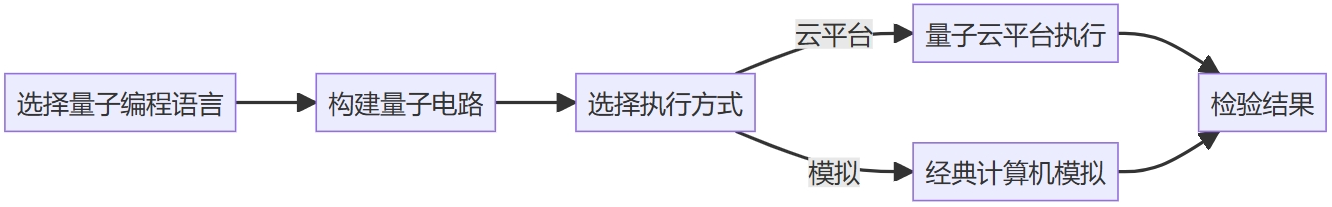
\includegraphics[width=0.9\textwidth]{figures/export.png}
    \label{fig_al}
\end{figure}

首先,需要选择一种量子编程语言,如Qiskit、Cirq、Q\#等。这些语言提供了构建量子电路、实现量子算法所需的工具和库。
之后,使用所选的量子编程语言,构建量子电路。量子电路由量子门组成,这些门定义了量子比特(qubits)之间的操作和相互作用。例如,在Qiskit中,可以使用Hadamard门和CNOT门来创建纠缠态。
构建量子电路后可以选择在真实的量子计算机上运行算法。如利用IBM Quantum、亚马逊Braket和微软Azure Quantum等平台,将构建的量子电路上传到云平台。这些平台提供量子模拟和量子硬件执行的能力,允许用户在真实的量子计算机上运行算法。
或者选择在经典计算机上模拟量子电路的运行,以验证量子算法的正确性和效率,该方法适用于小规模的量子电路。当然,由于是经典计算机上的模拟,其解决问题的实际速度不具有量子优势。
执行结束后分析算法的性能和结果。

本文通过Qiskit在计算机上模拟实现算法。
\subsection{Deutsch-Jozsa算法}
由David Deutsch和Richard Jozsa在1992年提出。该算法旨在解决所谓的Deutsch-Jozsa问题,即确定一个给定的二进制函数是常数函数还是均匀(balanced)函数。在经典计算中,确定函数是否为常数或平衡需要至少$2^{n-1}+1$次查询,其中N是函数可能输入的数量。然而,Deutsch-Jozsa算法只需一次函数查询就能解决这个问题,比任何经典算法都要快得多。
(常函数: 所有的$f(x)=0$或者1;
均匀(balanced)函数: 恰好一半$x$得$f(x) = 0$, 另一半$x$得$f(x) = 1$。)
\subsubsection{Deutsch-Jozsa算法描述}
Deutsch-Jozsa算法的量子线路如下:
\begin{define}{Deutsch-Jozsa算法量子线路}
    \begin{center}
    \begin{quantikz}[row sep=0.5cm, column sep=0.6cm]
        \lstick{$\ket{0}^{\otimes n}$} & \qw & \gate{H^{\otimes n}} & \qw & 
        \gate[2][2.0cm]{U_f}\gateinput[1]{$x$}\gateoutput[1]{$x$} & \qw & \gate{H^{\otimes n}} & \meter{} \\
        \lstick{$\ket{0}$} & \gate{X} & \gate{H} & \qw & \gateinput{$y$}\gateoutput{$y\oplus f(x)$} & \qw & \qw & \qw
    \end{quantikz}
    \end{center} 
\end{define}

$U_f$称为量子黑箱(Oracle),定义为:
$$
    U_f:\ket{x,y}\rightarrow\ket{x,y\oplus f(x)}
$$

若$|y\rangle = \frac{|0\rangle - |1\rangle}{\sqrt{2}}$,则有
$$
\begin{aligned}
    U_f : &|x\rangle \left( \frac{|0\rangle - |1\rangle}{\sqrt{2}} \right) \mapsto \left( \frac{U_f |x\rangle |0\rangle - U_f |x\rangle |1\rangle}{\sqrt{2}} \right)\\
    &= |x\rangle \left| 0 \oplus f(x) \right\rangle - |x\rangle \left| 1 \oplus f(x) \right\rangle\\
    &= |x\rangle \left( \frac{|0 \oplus f(x)\rangle - |1 \oplus f(x)\rangle}{\sqrt{2}} \right)
\end{aligned}
$$

当 $f(x) =$ 0 或 1 时,有
\[
\begin{cases} 
    f(x) = 0: & \frac{|0 \oplus f(x)\rangle - |1 \oplus f(x)\rangle}{\sqrt{2}} = \frac{|0\rangle - |1\rangle}{\sqrt{2}} \\ 
    f(x) = 1: & \frac{|0 \oplus f(x)\rangle - |1 \oplus f(x)\rangle}{\sqrt{2}} = \frac{|1\rangle - |0\rangle}{\sqrt{2}} = -\frac{|0\rangle - |1\rangle}{\sqrt{2}} 
\end{cases} 
\]

\[ \frac{|0 \oplus f(x)\rangle - |1 \oplus f(x)\rangle}{\sqrt{2}} = (-1)^{f(x)} \left( \frac{|0\rangle - |1\rangle}{\sqrt{2}} \right) \]

可见,$U_f$作用于 $|x\rangle \left( \frac{|0\rangle - |1\rangle}{\sqrt{2}} \right)$相当于从整体上添加了一个相位因子 $(-1)^{f(x)}$。

\[ U_f : |x\rangle \left( \frac{|0\rangle - |1\rangle}{\sqrt{2}} \right) \mapsto (-1)^{f(x)} |x\rangle \left( \frac{|0\rangle - |1\rangle}{\sqrt{2}} \right) \]

Deutsch-Jozsa算法工作过程如下:

1. 输入态: $|0\rangle^{\otimes n} \otimes |1\rangle$

2. $H^{\otimes n+1}$变换:

\[
|\psi_1\rangle = \left( \frac{|0\rangle + |1\rangle}{\sqrt{2}} \right)^{\otimes n} \otimes \frac{|0\rangle - |1\rangle}{\sqrt{2}} = \sum_{x \in \{0,1\}^n} \frac{|x\rangle\rangle}{\sqrt{2^n}} \otimes \frac{|0\rangle - |1\rangle}{\sqrt{2}}
\]

3. $\hat{U}$变换:

\[
|\psi_2\rangle = \hat{U}|\psi_1\rangle = \sum_{x \in \{0,1\}^n} \frac{(-1)^{f(x)}|x\rangle\rangle}{\sqrt{2^n}} \otimes \frac{|0\rangle - |1\rangle}{\sqrt{2}}
\]

4. $H^{\otimes n}$变换:

由 $H|y\rangle = \sum_{z=0,1} \frac{(-1)^{yz}}{\sqrt{2}} |z\rangle (y = 0 \text{和} 1)$ 得
\[
|\psi_3\rangle = \hat{U}|\psi_1\rangle = \sum_{x,z \in \{0,1\}^n} \frac{(-1)^{f(x) + x \cdot z}|z\rangle}{2^n} \otimes \frac{|0\rangle - |1\rangle}{\sqrt{2}}
\]

其中 $x \cdot z = \sum_{i=1}^{n} x_i z_i \mod 2$

5. 测量:

若 $f(x)$ 为常函数,则 $|z\rangle = |0\rangle^{\otimes n}$ 的系数为 $\sum_{x \in \{0,1\}^n} \frac{(-1)^{f(x)}}{2^n} = \pm 1$,此时 $|\psi_3\rangle = |0\rangle^{\otimes n} \otimes \frac{|0\rangle - |1\rangle}{\sqrt{2}}$,所以测量结果为所有量子位均为0。

若 $f(x)$ 为均匀函数,则 $|z\rangle = |0\rangle^{\otimes n}$ 的系数为零,所以测量结果不可能所有的量子位均为0。

\subsubsection{Deutsch-Jozsa算法Qiskit实现}
\bold{1.实现黑盒函数}

定义函数 \texttt{dj\_oracle(case, n)} 实现 Oracle,并将其构建为一个名为 Oracle 的自定义门,返回参数为新构建的自定义门的标识符。参数 $n$ 为输入量子比特的数目。参数 \texttt{case} 为字符串类型:当 \texttt{case} 为 \texttt{"constant"} 时,实现了常值函数;当 \texttt{case} 为 \texttt{"balanced"} 时,实现了平衡函数。
\begin{py}
\begin{lstlisting}
## oracle函数
def dj_oracle(case, n):
    oracle_qc = QuantumCircuit(n+1)
    # 平衡函数
    if case == "balanced":
        # [1,2**n)间的随机整数 b
        b = np.random.randint(1, 2**n)
        # 得到 b 对应的二进制字符串
        b_str = format(b, '0'+str(n)+'b')
        # 若b_str[qubit]为'1',则在q[qubit]上添加一个X门
        for qubit in range(len(b_str)):
            if b_str[qubit] == '1':
                oracle_qc.x(qubit)
        # 每个量子比特上添加 CNOT 门,q[n]为目标量子比特
        for qubit in range(n):
            oracle_qc.cx(qubit, n)
        # 若b_str[qubit]为'1',则在q[qubit]上添加一个X门
        for qubit in range(len(b_str)):
            if b_str[qubit] == '1':
                oracle_qc.x(qubit)

    # 常值函数
    if case == "constant":
        # 取随机整数0或1, 若为1,则在q[n]上添加一个X门
        output = np.random.randint(2)
        if output == 1:
            oracle_qc.x(n)

    oracle_gate = oracle_qc.to_gate()
    # 将量子线路 oracle_qc 封装为自定义门
    oracle_gate.name = "Oracle"
    return oracle_gate
\end{lstlisting}
\end{py}

例如,当$n=3$,$b=3$时利用以下代码可以得到平衡函数对应的量子线路:
\begin{py}
\begin{lstlisting}
from qiskit import QuantumCircuit 
import numpy as np
n = 3
oracle_qc = QuantumCircuit(n+1)
b = 3
b_str = format(b, '0'+str(n)+'b')
for qubit in range(len(b_str)):
    if b_str[qubit] == '1':
        oracle_qc.x(qubit)
for qubit in range(n):
    oracle_qc.cx(qubit, n)
for qubit in range(len(b_str)):
     if b_str[qubit] == '1':
        oracle_qc.x(qubit)
         
print(b_str)
oracle_qc.draw(output='mpl',filename='qc2.png')#获得png图片
\end{lstlisting}
\end{py}
\fig{平衡函数量子线路}{0.6}{code/qc2.png}
$q_0$,$q_1$ 和 $q_2$ 为输入量子比特,$q_3$ 为辅助量子比特。易知,输入为000、011、101、110时$q_3$进行了两次“非”,即$q_3$保持不变,对应$f(x)$为0。输入为111、001、100、010时$q_3$进行了一次或三次“非”,对应$f(x)$为1。故$f(x)$为平衡函数。

\bold{2.实现Deutsch-Jozsa算法的量子线路}
\begin{py}
\begin{lstlisting}
def dj_algorithm(oracle, n):
    dj_circuit = QuantumCircuit(n+1, n)
    # 设置输出量子比特
    dj_circuit.x(n)
    dj_circuit.h(n)
    # 设置输入寄存器
    for qubit in range(n):
        dj_circuit.h(qubit)
    # 添加 Oracle 门
    dj_circuit.append(oracle, range(n+1))
    # 输入寄存器各量子比特上添加 H 门
    for qubit in range(n):
        dj_circuit.h(qubit)
    # 测量输入寄存器
    for i in range(n):
        dj_circuit.measure(i, i)
    return dj_circuit



# 库函数输入
import numpy as np
from qiskit_aer import Aer
from qiskit import QuantumCircuit, transpile
from qiskit.visualization import plot_histogram

#实现4量子比特 Deutsch-Jozsa 算法量子线路
n = 4
oracle_gate = dj_oracle('constant', n)
# 平衡函数时,'constant'改为 'balanced'

dj_circuit = dj_algorithm(oracle_gate, n)
#dj_circuit.draw(output='mpl',filename='qc3.png')#获得png图片
\end{lstlisting}
\end{py}
\fig{4量子比特 Deutsch-Jozsa 算法量子线路图}{0.6}{code/qc3.png}

\bold{3.模拟运行Deutsch-Jozsa算法}
\begin{py}
\begin{lstlisting}
# 选择模拟器
simu = Aer.get_backend('aer_simulator')

# 编译运行电路
transpiled_dj_circuit = transpile(dj_circuit, simu)
results = simu.run(transpiled_dj_circuit).result()

# 获取测量结果
answer = results.get_counts(dj_circuit)
plot_histogram(answer)
\end{lstlisting}
\end{py}
测试结果测得 $|0000\rangle$ 的概率为 100\%对应 $f(x)$ 是常值函数。
测试结果测得 $|1111\rangle$ 的概率为 100\%对应 $f(x)$ 是平衡函数。(由于代码实现平衡函数时对其进行了限制,其他的态没有出现。)
\fig{常函数Deutsch-Jozsa 算法结果}{0.8}{code/const.png}
\fig{平衡函数Deutsch-Jozsa 算法结果}{0.8}{code/balanced.png}
\subsection{Grover搜索算法}
Grover搜索算法是由Lov Grover在1996年提出的一种量子算法,它主要用于解决无序数据库搜索问题,即在一个无序的数据库中寻找特定的元素。Grover算法被认为是继Shor算法之后的第二大量子算法,也是第一个被完整实验实现的量子算法。求解无序数据库搜索问题(假设只有一个目标搜索数据),经典算法所需的时间复杂度为\(\mathcal{O}(N)\),而Grover搜索算法所需的时间复杂度仅为\(\mathcal{O}(\sqrt{N})\),相比经典算法具有平方加速,展示了量子计算的强大性能。
\subsubsection{Grover搜索算法描述}
Grover算法的基本原理是利用量子叠加和量子干涉来放大目标态的概率振幅,同时抑制非目标态的概率振幅,这个过程被称为振幅放大。通过这种方式,Grover算法能够在多项式时间内找到一个无序数据库中的所有匹配项。
算法完成的任务: 一未知的黑盒$f :\{0,1\}^n\rightarrow\{0,1\}$, 找出使得$f(x) = 1$的$x$。

Grover算法的量子线路如下:
\begin{define}{Grover算法量子线路}
    \begin{center}
        \begin{quantikz}
            \lstick{$\ket{0}^{\otimes n}$} & \gate{H^{\otimes n}} & \gate[wires=2]{\hat{G}} & \gate[wires=2]{\hat{G}} & \qw \cdots & \gate[wires=2]{\hat{G}} & \meter{} \\
            \lstick{$\ket{1}$} & \gate{H} & \qw & \qw & \qw \cdots & \qw & \qw
        \end{quantikz}
    \end{center}

\begin{center}
    \begin{quantikz}
        \qw  & \gate[2][1cm]{\hat{G}} & \qw \\
        \qw & \qw & \qw
    \end{quantikz}$\Rightarrow$
    \begin{quantikz}
        \lstick{\ket{\psi}} & \qwbundle[n=2]{n} & \gate[2][1.7cm]{U_f}\gateinput[1]{$x$}\gateoutput[1]{$x$}  & \gate{2\ket{\psi}\bra{\psi} - I} & \qw \\
        \lstick{$\frac{\ket{0} - \ket{1}}{\sqrt{2}}$}& \qw & \gateinput{$y$}\gateoutput{$y\oplus f(x)$}  & \qw & \qw  \\
    \end{quantikz}    
\end{center}
\end{define}

Grover算法工作过程如下:

首先对初态为 $|0\rangle^{\otimes n}$,用 Hadamard 变换 $H^{\otimes n}$ 得到等权叠加态 $|\psi\rangle$(包含所有搜索问题的解与非搜索问题的解),即
\[
|\psi\rangle = \frac{1}{\sqrt{N}} \sum_{x=0}^{N-1} |x\rangle
\]

其中,$N = 2^n$。

此后,Grover算法连续多次执行G迭代操作。

Grover 的一次迭代分为以下四步:
\begin{enumerate}
    \item 执行 Oracle 操作($U_f$ 算符),将搜索问题的解对应的索引态增加相位因子 $-1$。
    \item Hadamard 变换 $H^{\otimes n}$。
    \item 相位变换:保持基态 $|0\rangle$ 的系数不变,其他基态的系数增加一个负号,对应的算符记为 $U_0 = 2|0\rangle\langle 0| - I$。
    \item Hadamard 变换 $H^{\otimes n}$。
\end{enumerate}

将2、3、4结合后的效果为
\[
U_{\psi} = H^{\otimes n} U_0 H^{\otimes n} = H^{\otimes n} (2|0\rangle\langle 0| - I) H^{\otimes n}
\]
\[
= 2H^{\otimes n} |0\rangle\langle 0| H^{\otimes n} - I = 2|\psi\rangle\langle\psi| - I
\]

于是,Grover 一次迭代的操作算符 $G$ 等价于
\[
G = U_{\psi} U_f = (2|\psi\rangle\langle\psi| - I) U_f
\]

通过上面的迭代,测量塌缩到索引的态的概率增大,多次迭代后完成搜索。
\subsubsection{Grover算法Qiskit实现}
通过Qiskit实现$\ket{000},\ket{001},\ket{100},\ket{010},\ket{011},\ket{110},\ket{101},\ket{111}$找$\ket{111}$的Grover算法。

Qiskit实现:

\bold{1.实现黑盒函数}

\begin{py}
\begin{lstlisting}
# 初始化
import numpy as np
# 导入 Qiskit 库
from qiskit import QuantumCircuit, transpile, quantum_info
from qiskit_aer import QasmSimulator
from qiskit import ClassicalRegister, QuantumRegister
from qiskit.visualization import plot_histogram

# 设置量子比特数量
n = 3

# 定义 Oracle 函数,用于标记特定的量子态 |111>
def Oracle():  
    oc = QuantumCircuit(n) 
    # 使用H门和CCX门(受控非门)来实现 CZ 门的效果
    oc.h(2)  # 对第2个量子比特应用Hadamard门
    oc.ccx(0, 1, 2)  # 应用受控非门
    oc.h(2)  # 再次对第2个量子比特应用Hadamard门
    return oc

\end{lstlisting}
\end{py}

\bold{2.实现振幅放大}

\begin{py}
\begin{lstlisting}
# 定义扩散算子函数,用于实现幅度放大
def A(nb): 
    ac = QuantumCircuit(nb)
    ac.h(range(nb))  # 对所有量子比特应用Hadamard门
    ac.x(range(nb))  # 对所有量子比特应用X门(非门)
    # 执行多控制Z门
    ac.h(nb-1)  # 对最后一个量子比特应用Hadamard门
    ac.mcx(list(range(nb-1)), nb-1)  # 多控制Z门
    ac.h(nb-1)  # 再次对最后一个量子比特应用Hadamard门
    ac.x(range(nb))  # 对所有量子比特应用X门
    ac.h(range(nb))  # 对所有量子比特再次应用Hadamard门
    return ac
\end{lstlisting}
\end{py}

\bold{3.实现Grover算法}
\begin{py}
\begin{lstlisting}
    # 创建量子电路
    qc = QuantumCircuit(n)
    qc.h(range(n))  # 对所有量子比特应用Hadamard门
    
    # 构建 Oracle 和幅度放大电路
    OA = QuantumCircuit(n)
    # 将Oracle函数内的内容组合到OA电路中
    OA.compose(Oracle(), inplace=True)  
    # 将扩散算子组合到OA电路中
    OA.compose(A(n), inplace=True)  
    # 将OA电路组合到qc电路中
    qc.compose(OA, inplace=True)     
    # 绘制电路图
    qc.draw(output='mpl',filename='grover_circuit.png')
\end{lstlisting}
\end{py}
\fig{Grover算法量子电路}{0.8}{code/grover_circuit.png}

\bold{4.模拟运行}
\begin{py}
\begin{lstlisting}
qc.save_statevector()  # 保存量子电路的状态向量


simulator = QasmSimulator()
compiled_circuit = transpile(qc, simulator)
job = simulator.run(compiled_circuit, shots=1000)
result = job.result()  # 获取运行结果
out_state = result.get_statevector()  # 获取状态向量
counts = result.get_counts()  # 获取测量结果的计数
# 反转字典 counts 中的字符串并存储到新字典answer中
answer = {}
for str in counts:
    answer[str[::-1]] = counts[str]  
# 绘图
plot_histogram(answer).savefig('groverout.png') 
\end{lstlisting}
\end{py}
\fig{Grover算法输出结果}{0.5}{code/groverout.png}
从输出结果不难看出,$\ket{111}$的振幅(出现的概率)被明显放大,代码实现了Grover算法的功能。
\section{总结}
\subsection{研究成果概述}

\begin{enumerate}[leftmargin=0pt]
    \item 量子计算基础原理 \\
    本文首先介绍了量子计算的基本概念,包括量子位(qubit)的特性、量子门的分类与作用以及量子线路的设计原理。量子位作为量子计算的基本信息单元,具有量子叠加和量子纠缠的特性,使得量子计算能够实现并行计算,从而在某些特定问题上展现出超越经典计算的潜力。量子门作为量子计算中的基本操作单元,通过幺正矩阵表示的线性变换改变量子位的状态,是实现量子算法的基础。量子线路则是通过一系列量子门操作量子位,实现量子算法的图形化表示方法。
    
    \item 量子计算的物理实现 \\
    本文简要总结了离子阱量子计算和超导量子计算这两种主流的量子计算物理实现方式。离子阱量子计算利用囚禁离子作为量子比特,具有高保真度、长相干时间和精确控制等优势,但面临量子比特扩展性和量子门保真度提升的挑战。超导量子计算则通过设计具有特定能级结构的超导电路实现量子比特,具有可配置性强、操作灵活的特点,但受到噪声与退相干问题、可扩展性限制以及高昂成本的制约。通过对这两种技术的分析,本文揭示了量子计算从理论到实践的关键环节,并指出了当前技术面临的挑战和未来发展方向。
    
    \item 量子算法及编程实现 \\
    本文通过Qiskit框架在经典计算机上对Deutsch-Jozsa算法和Grover搜索算法进行了模拟实现。Deutsch-Jozsa算法能够在一次函数查询内判断一个二进制函数是常数函数还是平衡函数,相比经典算法具有显著的效率优势。Grover搜索算法则为无序数据库搜索问题提供了平方加速的解决方案,展示了量子计算在解决实际问题中的强大性能。通过编程实践,本文不仅验证了这些量子算法的正确性和有效性,还展示了量子编程的基本方法和流程,为量子算法的进一步研究和应用提供了实践指导。
\end{enumerate}

\subsection{研究意义与展望}

量子计算作为一种新兴的计算范式,具有巨大的发展潜力和广泛的应用前景。本文的研究不仅为读者提供了一个全面的量子计算入门框架,还通过实际的编程实践,加深了对量子计算原理和算法的理解。量子计算的发展有望在密码学、化学、材料科学、人工智能等领域带来革命性的变化。例如,量子计算能够高效地模拟量子系统,为新材料的设计和药物研发提供强大的计算支持;量子算法的加速特性则可能为大数据处理和机器学习带来新的突破。

然而,量子计算的发展仍面临诸多挑战。物理实现方面,量子比特的扩展性、量子门的保真度、量子比特的相干时间以及量子计算的容错性等问题亟待解决。在软件和应用层面,量子编程语言的开发和量子算法的优化也是当前研究的重点。未来,随着量子计算技术的不断进步,量子计算有望从实验室走向实际应用,为解决复杂计算问题提供全新的解决方案。

\subsection{结论}

本文通过对量子计算的基本原理、物理实现方式以及量子算法的编程实现的系统研究,展示了量子计算的强大潜力和广阔的应用前景。量子计算的发展不仅需要物理学家和工程师在硬件层面的突破,也需要计算机科学家和数学家在软件和算法层面的创新。随着量子计算技术的不断成熟,我们有理由相信,量子计算将在未来的科技发展中扮演重要角色,为人类社会带来深远的影响。

\appendix %附录部分

\section{量子编程语言与量子云平台}
随着量子计算不断“出圈”,人们对其也越加重视,许多开发库与工具应运而生。这里对部分典型的量子编程语言及量子云平台进行介绍。
\subsection{量子编程语言}
\textbf{1. Cirq (https://github.com/quantumlib/Cirq)}

Cirq是由Google开发的开源量子计算编程框架,它专注于量子算法的开发和演示,并提供了一套灵活的工具和库,可以在量子计算机上进行量子计算的模拟和实验。Cirq的主要特点包括面向研究和教育、灵活的模拟、可扩展性以及强大的调试工具。它支持多种不同类型的量子计算架构,包括通用量子计算和量子模拟,这使得用户可以自由地在不同的硬件平台和算法中进行开发和测试。

\textbf{2. Qiskit (https://www.ibm.com/quantum/qiskit)}

Qiskit是一个由IBM开发的开源量子计算软件开发框架,旨在利用当今的量子处理器进行研究、教育和商业活动。它支持多种量子计算平台,包括量子模拟器和真实量子计算机。Qiskit的目标是使开发者能够利用量子计算的潜力,并为其提供必要的工具。
Qiskit的主要组件包括:

\begin{paralist}
    \item Qiskit Terra:提供基本的构建块和API,允许用户构建量子电路。
    \item Qiskit Aer:用于模拟量子电路和量子计算的工具。
    \item Qiskit Ignis:用于量子误差校正和噪声研究的组件。
    \item Qiskit Aqua:用于应用于量子算法的高层次接口。
    \item Qiskit Nature:专注于化学和物理的量子应用。
\end{paralist}


\textbf{3. Q\# (https://learn.microsoft.com/zh-cn/azure/quantum/qsharp-overview)}

Q\# 是由 Microsoft 开发的专门用于量子计算的高级开源编程语言,它包含在 Quantum 开发工具包(QDK)中。Q\# 旨在帮助开发人员利用量子计算的潜力来解决复杂问题。它提供声明式编程方法,集成开发环境,丰富的库和工具,可扩展性和互操作性,量子模拟器和开源支持。Q\# 支持硬件不可知的量子算法开发,使得编写的量子程序可以在不同的量子计算机和模拟器上运行。

\textbf{4. QPanda (https://qcloud.originqc.com.cn/zh/programming/QPanda)}

QPanda是由本源量子开发的开源量子计算框架,它可以用于构建、运行和优化量子算法。QPanda 作为本源量子计算系列软件的基础库,为OriginIR、Qurator、量子计算服务提供核心部件。QPanda是一种功能齐全、运行高效的量子软件开发工具包,它是一款开源的量子计算框架,可以用于构建、运行和优化量子算法。QPanda提供了丰富的量子计算编程基础组件,包括量子比特和量子门操作,开发者可以使用这些组件来构建复杂的量子算法,从简单的量子门序列到更复杂的量子电路。这些基础组件为开发者提供了构建量子计算任务所需的核心工具。此外,QPanda还提供了高性能量子虚拟机,允许开发者在经典计算机上进行高效的量子模拟,使开发者能够在不依赖实际量子硬件的情况下测试和优化他们的算法。

\subsection{量子云平台}
\textbf{1. IBM Quantum  (https://www.ibm.com/quantum)}

IBM Quantum 允许用户在 IBM 的真实量子计算机上运行量子算法。它提供了一个用户友好的界面,以及一套量子编程工具,如 Qiskit,来设计和测试量子电路。IBM Quantum旨在促进量子计算的研究和教育,使量子计算对更广泛的用户群体开放。

\textbf{2. Amazon Braket (https://aws.amazon.com/braket/)}

Amazon Braket 是一项完全托管的量子计算服务,旨在帮助加快量子计算的科学研究和软件开发。它允许用户轻松处理不同类型的量子计算机和电路模拟器,使用一组一致的开发工具。Braket 提供了对超导、俘获离子和中性原子设备的支持,以及量子硬件研究的界限突破。此外,它还提供了软件开发工具包(SDK)、简单的定价和工作流管理,以及开源软件的开发支持。

\textbf{3. Azure Quantum (https://azure.microsoft.com/zh-cn/products/quantum/)}

Azure Quantum 是微软提供的量子云计算服务,构建在可信赖、可扩展且高度安全的 Azure 平台上。它包括来自微软和合作伙伴的多样化量子硬件和软件解决方案,提供了一个开放、灵活的环境,适应用户需求,加速进展并确保技术的未来发展。Azure Quantum 支持 Cirq、Qiskit 和 Q\# 等编程语言,允许用户在多个平台上创建和运行算法,同时保留针对特定系统进行调整的能力。

\textbf{4. 本源量子云 (https://qcloud.originqc.com.cn/zh/home)}

本源量子云提供真实量子计算、量子计算模拟器和超-量混合计算后端接入,为开发者提供基础软件与开发工具,为生物化学、金融科技、大数据、机器学习等先进企业提供行业应用服务
\section{Qiskit的安装及基本使用方法}
\label{附录A}
\subsection{Qiskit的安装}
\textbf{Qiskit的安装要求:}

Python版本:建议使用Python 3.6及以上版本。这是Qiskit运行的基础环境,确保Python版本符合要求可以避免安装过程中出现兼容性问题。

操作系统:Qiskit支持64位操作系统,如Ubuntu 16.04、macOS 10.12.6、Windows 7及以上版本。

基础函数库:Qiskit安装过程中可能需要一些基础函数库,如Numpy等。

\subsubsection{下载并安装Anaconda}
\begin{paralist}
    \item 下载Anaconda:进入官网下载(https://www.anaconda.com/download)

    \item 安装conda 
\end{paralist}
\subsubsection{创建虚拟环境并安装Qiskit}
\begin{paralist}
    \item 虚拟环境的创建:打开Anaconda Prompt输入并运行\textsf{conda create -n py python=3.8}
    \item 激活虚拟环境:输入并运行\textsf{conda activate py}
    \item 安装Qiskit:在虚拟环境下输入并运行\textsf{pip install qiskit[visualization]}(遇到网络问题可以配置使用镜像源)
\end{paralist}
\subsubsection{Jupyter Notebook使用}
在创建好的虚拟环境中输入:
\begin{paralist}
    \item \textsf{conda install ipykernel}
    \item \textsf{ipython kernel install --user --name=pykernel}
\end{paralist}

在Anaconda安装目录下打开Jupyter Notebook,点击New且选择pykernel创建ipynb文件,即可开始编写、运行程序。
\figu{0.4}{figures/ju.png}
\subsection{Qiskit的基本使用方法}
Qiskit能实现多个功能。下面主要介绍如何创建量子线路并绘制、如何模拟器运行量子线路。

\bold{1.创建、绘制量子线路}

Qiskit 创建与绘制量子线路的主要步骤如下:

\begin{py}
\begin{lstlisting}
#1.导入库
from qiskit import(QuantumCircuit,transpile)
from qiskit_aer import Aer
from qiskit.visualization import plot_histogram
#2.创建量子线路
circuit = QuantumCircuit(2,2)#创建两个经典位与量子位
circuit.h(0)#在第0个量子位上添加H门
circuit.cx(0,1)#添加受控非门,控制位为0,目标位为1
circuit.measure([0,1],[0,1])
#(qubit, cbit)将qubit测量结果存储到cbit中
#3.绘制量子线路
circuit.draw(output='mpl',filename='qc.png')#获得png图片
\end{lstlisting}
\end{py}
\fig{输出的量子线路图}{0.6}{code/qc.png}

\bold{2.模拟器运行}

QasmSimulator和StatevectorSimulator为Qiskit中两类常用的模拟器,它们的特点如下:
\begin{paralist}
    \item QasmSimulator:模拟量子线路的多次运行并返回测量结果的概率分布。
    \item StatevectorSimulator:返回量子线路的最终状态向量。主要用于分析量子线路的量子态,不涉及测量操作。
\end{paralist}

QasmSimulator使用示例:
\begin{py}
\begin{lstlisting}
#QasmSimulator使用示例
from qiskit import QuantumCircuit, transpile
from qiskit_aer import Aer
from qiskit.visualization import plot_histogram

# 创建量子线路
qc = QuantumCircuit(2, 2)
qc.h(0)
qc.cx(0, 1)
qc.measure([0, 1], [0, 1])

# 选择QasmSimulator
simulator = = Aer.get_backend('qasm_simulator')

# 编译电路
transpiled_circuit = transpile(qc, simulator)

# 运行电路并获取结果
job = simulator.run(transpiled_circuit, shots=1024)
result = job.result()

# 获取测量结果
counts = result.get_counts(qc)
print("实验结果:", counts)

# 可视化
out = plot_histogram(counts)
out.savefig('out.png')
\end{lstlisting}
\end{py}

\fig{QasmSimulator使用示例输出结果}{0.6}{code/out.png}
输出结果与\( |\Phi^{+}\rangle = \frac{1}{\sqrt{2}} (|00\rangle + |11\rangle) \),$|00\rangle$与$|11\rangle$出现概率为$50\%$对应。

StatevectorSimulator使用示例:

\begin{py}
\begin{lstlisting}
#StatevectorSimulator使用示例
from qiskit import QuantumCircuit, transpile
from qiskit_aer import Aer
from qiskit.visualization import plot_state_city

# 创建量子线路
qc = QuantumCircuit(2)
qc.h(0)
qc.cx(0, 1)

# 选择StatevectorSimulator
simulator = Aer.get_backend('statevector_simulator') 


# 编译电路
transpiled_circuit = transpile(qc, simulator)

# 运行电路并获取结果
job = simulator.run(transpiled_circuit)
result = job.result()

# 获取状态向量
statevector = result.get_statevector(qc)

#可视化
out=plot_state_city(statevector)
out.savefig('out1.png')
\end{lstlisting}
\end{py}
\fig{StatevectorSimulator使用示例输出结果}{0.8}{code/out1.png}
输出结果与 \( |\Phi^{+}\rangle = \frac{1}{\sqrt{2}} (|00\rangle + |11\rangle) \) 的密度矩阵一致,即

\[
\rho_{\Phi^{+}} = |\Phi^{+}\rangle \langle \Phi^{+}|
= \begin{bmatrix} \frac{1}{\sqrt{2}} \\ 0 \\ 0 \\ \frac{1}{\sqrt{2}} \end{bmatrix} \begin{bmatrix} \frac{1}{\sqrt{2}} & 0 & 0 & \frac{1}{\sqrt{2}} \end{bmatrix}
= \frac{1}{2} \begin{bmatrix} 1 & 0 & 0 & 1 \\ 0 & 0 & 0 & 0 \\ 0 & 0 & 0 & 0 \\ 1 & 0 & 0 & 1 \end{bmatrix}
\]

除以上两个模拟器外,Qiskit中还有模拟器Uintary Simulator。通过UnitarySimulator,可以方便地得到整个量子线路对应的单位矩阵,对于理论分析和验证量子线路的正确性非常有用。使用方法与上面类似。
\begin{py}
\begin{lstlisting}
#UnitarySimulator使用示例
from qiskit import QuantumCircuit, transpile
from qiskit_aer import Aer

# 创建量子线路
qc = QuantumCircuit(2)
qc.h(0)
qc.cx(0, 1)

# 选择 unitary_simulator
simulator = Aer.get_backend('unitary_simulator')

# 编译电路
transpiled_circuit = transpile(qc, simulator)

# 运行电路并获取结果
job = simulator.run(transpiled_circuit)
result = job.result()

# 获取单位矩阵
unitary = result.get_unitary(qc)
print("单位矩阵:\n", unitary)  
\end{lstlisting}
\end{py}
\fig{UnitarySimulator使用示例输出结果}{0.8}{figures/uni.png}
% 生成参考文献列表
\addcontentsline{toc}{section}{参考文献}%为了加入目录
\nocite{*} %不引用
\bibliographystyle{plain}  % 选择参考文献的格式
\bibliography{bib/references}  % 引用 BibTeX 文件

\end{document}

